\subsection{Электронное строение (с позиций ММО) бисциклопентадиенильных комплексов переходных металлов}

\subsubsection*{Металлоцены}
Ферроцен - устойчив кинетически, но не термодинамически. Соединения устойчивы в довольно широком диапазоне: 
$$Cp_2V, Cp_2Cr, Cp_2Mn, Cp_2Fe, Cp_2Co, Cp_2Ni$$

Все эти соединения идентичны структурно, по составу тоже, только иимеют разные длины связи.

$$Cp_2Fe - D_{5h}$$

\begin{figure}[H]
\centering
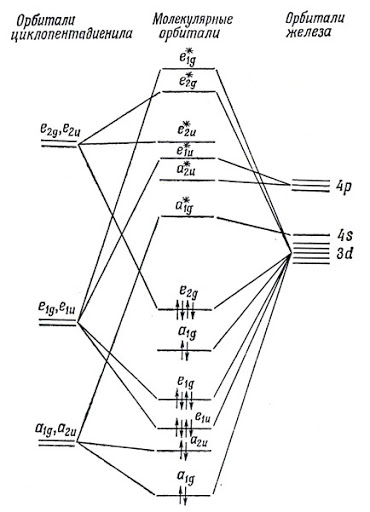
\includegraphics[scale=.500]{images/CP.jpg}
\caption{}
\label{}
\end{figure}

\begin{itemize}

\item Всего 59 орбиталей, из них 40 - обеспечивают связи в кольце и не учитаваются при рассмотрении

\item Сильно переурывание по $\pi$($Cp(e_1) - d_{xz}, Cp(e_1) - d_{yz}$), почти равно нулю $\sigma$($Cp(e_1) - d_z^2$).

\item Слабосвязывающие орбитали: $e_2$, $e_1$, из-за этого устойчивы $Cp_2V(16e), Cp_2Cr(16e), Cp_2Mn(17e)$

\item $Cp$ - $\sigma$-донор, сильный $\pi-$донор, слабый $\sigma-$акцептор.
\end{itemize}
